\chapter{Heaven}

\section{Requirements}


\section{Architecture}
\subsection{Streamer}
\subsection{Result Collector}
\subsection{RSP Engine}
\subsection{Test Stand}
\subsection{Analyser}
\section{Implementation}
\subsection{Streamer - RDF2RDFStream}
\subsection{Result Collector}
\subsection{RSP Engine - Esper Integration}
\subsection{Test Stand}
\subsection{Analyser}

\section{Baselines}
\subsection{Time Control}
\subsection{Stream Model}
\subsection{Reasoning}


Esempio di figura

\begin{figure}[ht]
\centerline{\epsfig{file=esempio.ps, width=12 true cm}}
\caption{Didascalia esempio di figura.}
\label{fig:esempio}
\end{figure}

Esempio di equazione

\begin{equation}
\dot V_4= - k_v \lambda (z_1- \varepsilon \lambda z_3)^T(z_1-
\varepsilon \lambda z_3).
\end{equation}
